\documentclass[a4paper,12pt]{scrreprt}
\usepackage[T1]{fontenc}
\usepackage[utf8]{inputenc}
\usepackage[ngerman]{babel}
\usepackage[table]{xcolor}
% http://ctan.org/pkg/xcolor
\usepackage{tabu}
\usepackage{graphicx}
\usepackage{lmodern}
\usepackage{hyperref}
\usepackage{geometry}
\geometry{verbose,a4paper,tmargin=20mm,bmargin=40mm,lmargin=40mm,rmargin=30mm}



\begin{document}


%\titlehead{Kopf} %Optionale Kopfzeile
\author{Alexander Rieppel} %Zwei Autoren
\title{Transportlogistik} %Titel/Thema
\subject{Betriebs- und Informationsmanagement} %Fach
\subtitle{Ausarbeitung} %Genaueres Thema, Optional
\date{\today} %Datum
\publishers{5AHITT} %Klasse
{\Huge }

\maketitle
\tableofcontents


\chapter{Einführung}
	Der Begriff Transportlogistik beschreibt die Lieferung und Beförderung von Gütern, zwischen verschiedenen Orten innerhalb von Transportnetzwerken. Dieser Teilbereich der Logistik ist durch den heutigen Wohlstand entstanden, in dem sich Unternehmen auf ihre Kernkompetenzen konzentrieren und darüber hinausgehende Dienstleistungen und Produkte europaweit und international einkaufen. Die Planung und Optimierung, Ausführung, Überwachung und Steuerung der damit verbundenen Güterströme ist Aufgabe der Transportlogistik. Neben dem Transport von Waren als solches wird auch die Be- und Entladung zur Transportlogistik gezählt.\\
	
	Das Problem Güter von A nach B zu bringen ist für jeden Unternehmer eine Herausforderung. Prinzipiell ist es dabei egal, ob die Ware per LKW, Zug, Schiff, Flugzeug, Pipeline, etc. transportiert wird. Es geht rein darum, dass die Ware ankommt, sie möglichst unbeschadet ankommt und vor allem schnell am Ziel ist. Auch der Kostenfaktor spielt dabei eine große Rolle und auch ökologische Nachhaltigkeit gewinnt zunehmend an Bedeutung.\\
	
	Obwohl es im Prinzip egal ist womit transportiert wird, ist der am meisten genutzte Verkehrsträger zur Güterbeförderung, speziell hierzulande, die Straße. Zu den entscheidenden Gründen zählt die Netzbildungsfähigkeit des LKW, der jede Quelle und Senke flexibel erreichen kann. Die Stärke von Schiene und Binnenwasser-straße liegen in dem effizienten Transport von Massengütern über längere Strecken. Für die besonders langen Distanzen im internationalen Gütertransport werden das Seeschiff für große Volumina und das Flugzeug eher für besonders eilige oder wertvolle Fracht genutzt. Neben der reinen Beförderung als offensichtlichste transportlogistische Funktion erfordern die Ver- und Entsorgung von Industrie- und Handelsunternehmen weitere Leistungen, wie die Lagerhaltung für die zeitliche Überbrückung zwischen Fertigung und Absatz, den Umschlag im Rahmen des Verkehrsmittelwechsels und die Kommissionierung zur Vereinzelung nachgefragter Mengen. Hinzu kommen verstärkt auch Tätigkeiten, die einen zusätzlichen Mehrwert am Gut schaffen, wie die Montage von Teilen zu Modulen, die Aufarbeitung von Produkten, ihre Etikettierung oder Sequenzierung.\\
	
	Die Transportlogistik wurde lange Zeit auf reine Transport-, Lager- und Umschlagtätigkeiten reduziert. In der jüngsten Vergangenheit hat sich die Transportlogistik von einer ausführenden Funktion zu einem entscheidenden Wettbewerbsfaktor in der Gestaltung und Steuerung nationaler und internationaler Wertschöpfungsketten entwickelt. Unter hochrangigen Persönlichkeiten österreichischer und internationaler Firmen finden sich zunehmend Logistiker. Auch hat Logistik zunehmend eine hohe Relevanz in Politik und Gesellschaft.
	
	Dies zeigt auch, dass die Gütertransportlogistik steigenden
	Anforderungen unterliegt, durch einen stetigen Anstieg gekennzeichnet ist, aber auch eine Fülle von Gestaltungsmöglichkeiten bietet. Dies belegt die Bedeutung der Transportlogistik mit der Folge, dass sich Gesellschaft, Wirtschaft und Wissenschaft intensiv mit Fragestellungen auf diesem Gebiet auseinander setzen müssen.\\\\
	Zu den Zielen der Transportlogistik gehören:
	\begin{itemize}
	\item Effektivität - die Aufgaben werden erfüllt
	\item Effizienz - die Aufgaben werden mit einem günstigen Kosten-Nutzen Verhältnis erfüllt
	\item Sicherheit - Gegen technische Störungen, Unfälle, etc. wird vorgebeugt
	\item Robustheit - Transportketten arbeiten auch im Fall von Störungen und Auftragsschwankungen zuverlässig
	\item Nachhaltigkeit - Neben ökonomischen Belangen sind ökologische und soziale Interessen zu berücksichtigen
	\item Wirtschaftlichkeit - Die Kosten sind angemessen und die erzielbaren Erträge decken für alle beteiligten die Aufwände
	\end{itemize}
	
	\begin{center}

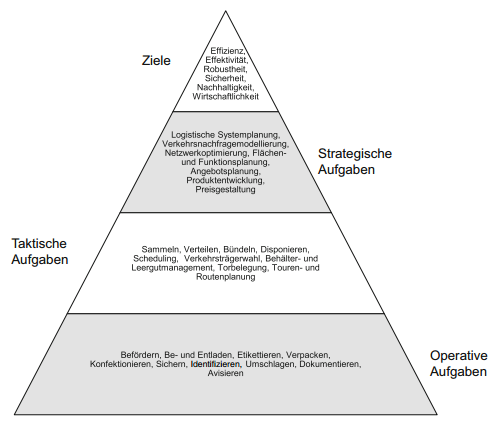
\includegraphics[width=1\linewidth]{./Bilder/Ziele_Transportlogistik}
\end{center}

	\chapter{Wirtschaftliche Aspekte der Transportlogistik}
	
	Die Logistik ist für sämtliche Industriebranchen ein maßgeblicher Faktor. Insbesondere sind die Chemiebranche, die Stahlbranche, die Automobilbranche und das verarbeitende Gewerbe, von einem reibungslosen Ablauf der Logistik abhängig, um ihre Wertschöpfungskette aufrecht erhalten zu können. Die erforderlichen Transporte erstrecken sich über die ganze Welt. Sie finden zwischen verschiedenen Partnern der Wertschöpfungskette, von der Rohstoffgewinnung, über die Verarbeitung und den Handel bis hin zum Endkunden statt. Die Partner innerhalb der Wertschöpfungskette können verschiedenen Industrien angehören. Beispielsweise ist die Stahl- und Metallindustrie ein wesentlicher Zulieferer der Automobilindustrie.\\
	
	Die Transportlogistik nimmt im Vergleich international eine Schlüsselposition ein. Mit einem weltweiten Marktvolumen von 4.200 Mrd. Euro ist die Logistik nach der Automobilindustrie und dem Maschinenbau die drittgrößte Branche. Alleine in Europa erzielte die Logistik 2009 ein Martvolumen von 880 Mrd. Euro. Von diesen erbrachten Logistikleistungen entfallen - gemessen in Wertschöpfung - mehr als ein Drittel auf das Transportgeschäft. Damit ist die Transportlogistik eine wichtige Branche mit bedeutender Zukunftsaussicht, wobei durch die Schwankungen am Markt und die Wettbewerbsintensität nicht immer die gewünschten Rendite erzielt werden.\\
	
	\chapter{Logistikdienstleister}
	Ein Logistikdienstleister ist ein Unternehmen, dessen Tätigkeitsschwerpunkt in der Erbringung von logistischen Dienstleistungen für andere Unternehmen liegt. Diese leistungsbeziehenden Unternehmen treten als Auftraggeber des Logistikdienstleisters auf und werden unter dem Begriff „Verlader“ zusammengefasst. Zu ihnen zählen Industrie-, Handels- und Dienstleistungsunternehmen, welche als Lieferant oder Konsument von Gütern Logistikleistungen nachfragen. Im nachfolgenden Abschnitt werden ausgewählte Formen von Logistikdienstleistern aufgeführt und erklärt.
	\section{Transportunternehmen}
	Die auch als Carrier bezeichneten Transportunternehmen sind	auf die reine Beförderung von Gütern spezialisiert. Dabei greifen sie üblicherweise auf betriebseigene Transportmittel zurück. Transportunternehmen leisten somit einen räumlichen Ausgleich als isoliertes Element einer Lieferkette. 
	\section{Lagerunternehmen}
	Gewerbliche Unternehmen, welche schwerpunktmäßig das Lagergeschäft betreiben, werden als Lagerhalter bezeichnet. Gegenstand des Lagergeschäfts ist, einen zeitlichen Ausgleich zu schaffen, beispielsweise zwischen Produktions- und Absatzdatum. Mit der Zeitüberbrückung steuern Lagerunternehmen eine ausgewählte Funktion zum Betrieb einer gesamten Lieferkette bei. 
	\section{Speditionen}
	Unternehmen, welche nach Abschluss eines Speditionsvertrags die Versendung von Gütern für Dritte besorgen, heißen Speditionen. Die zentrale Aufgabe eines Spediteurs besteht dabei in der Organisation der Beförderung. Diese umfasst
	\begin{itemize}
	\item die Bestimmung des Beförderungsmittels und des Beförderungsweges,
	\item die Auswahl ausführender Unternehmer, den Abschluss der für die Versendung erforderlichen Fracht-, Lager- und Speditionsverträge sowie die Erteilung von Informationen und Weisungen an die ausführenden Unternehmer und
	\item die Sicherung von Schadenersatzansprüchen des Versenders.
	\end{itemize}
	Über die Organisation der Beförderung hinaus kann der Versender den Spediteur mit weiteren, damit verbundenen Leistungen betrauen, wie z. B. die Versicherung und Verpackung der Güter, ihre Kennzeichnung und die Zollbehandlung. Sofern vereinbart ist der Spediteur dabei lediglich zum Abschluss der Verträge verpflichtet, die zur Erbringung dieser Leistungen erforderlich sind. Mit diesen Aufgaben bekleidet der Spediteur in erster Linie eine planende und steuernde Position für ein logistisches Teilsystem. Durch die Annahme des verladerseitig erteilten Speditionsauftrags und die Auswahl, Beauftragung und Kontrolle der abwickelnden Unternehmen nimmt der Spediteur die Rolle des Vermittlers zwischen Nachfrager und Anbieter von logistischen Dienstleistungen ein.
	\section{Kontraktlogistikdienstleister}
	Entscheidet sich ein Industrie- oder Handelsunternehmen	zur Auslagerung mehrerer, bislang intern erbrachter Logistikfunktionen, so beauftragt es einen Systemdienstleister. Dieser wird als Kontraktlogistikdienstleister oder mit dem englischsprachigen Begriff Third-Party-Logistics-Provider – abgekürzt 3PL – bezeichnet. Die fremdvergebenen Funktionen können die gesamte Logistikkette oder daraus ausgewählte Abschnitte, z. B. die Beschaffungs- oder Distributionslogistik, umspannen. Der Kontraktlogistikdienstleister übernimmt somit von seinem Verlader ein komplettes, unternehmensindividuelles Logistiksystem. Dementsprechend handelt es sich bei den zur Funktionserfüllung notwendigen Leistungen um integrierte Dienstleistungsbündel. Diese beinhalten zum einen das Management und die Ausführungen der Basisleistungen Transport, Umschlag und/oder Lagerhaltung. Zum anderen sind damit verbundene Zusatzleistungen wie Verpackung, Montagetätigkeiten und Installationsarbeiten, Bestandsmanagement sowie Tracking und Tracing inbegriffen. Bedingt durch diese funktionale Breite besitzen die Leistungen des Kontraktlogistikdienstleisters im Vergleich zu den klassischen Einzelleistungen der Transport- und	Lagerunternehmen einen weit komplexeren Charakter. Für die Produktion der Leistungen verfügen Kontraktlogistikdienstleister über eigene Ressourcen. Sie zählen daher zu den sogenannten asset-based Dienstleistern.
	
	\chapter{Verkehrsträger im Güterverkehr}
	Transportmittel sind grundsätzlich Fortbewegungsmittel zur Beförderung von Personen oder Gütern innerhalb von Verkehrsträgern. Dies können z.B. der LKW im Straßenverkehr, die Bahn im Schienenverkehr, das Binnenschiff in der Binnenschifffahrt oder das Flugzeug im Luftverkehr sein. Da der Schwerpunkt dieser Arbeit auf dem Transport von Gütern liegt, werden Verkehrsmittel des Personenverkehrs, hier nicht weiter betrachtet.\\
	
	Die einzelnen Transportmittel weisen verschiedenste Vor- und Nachteile auf. Aufgrund der zuvor beschriebenen Flächendeckung ist der LKW das flexibelste Transportmittel. Zudem ist für die Führung eines LKWs die geringste Ausbildungszeit zu absolvieren. Daher eignet er sich insbesondere für kurze Strecken, eilbedürftige Güter und für den Flächenverkehr. Ein Nachteil dieses Transportmittels liegt in der zu anderen Transportmitteln, wie Eisenbahn und Binnenschiff, vergleichsweise  geringen Gütermenge, die ein LKW aufnehmen kann. Auch in der Umweltbilanz schneidet ein LKW, entsprechend schlechter ab. Diese liegen pro 100tkm bei 4.1l beim LKW, 1.7l bei der Eisenbahn und 1,3l beim Binnenschiff. Die besseren Verbrauchswerte liegen unter anderem an der erheblich geringeren Reisegeschwindigkeit von Schiff und Bahn. Hierdurch eignen sich Schiff und Bahn in der Regel nicht für eilbedürftige Güter. Auch sind sie durch die kleineren Netze nicht für den Flächenverkehr geeignet. Die spezifischen Vorteile der Verkehrsmittel Eisenbahn und Binnenschiff liegen unter anderem in der Affinität zu Massengütern. Die jeweiligen Vorteile werden später noch genauer im Unterkaptitel Kombinierter Verkehr behandelt und vereint ohne dabei die Nachteile der Transportmittel in Kauf nehmen zu müssen.
	\section{Straßengüterverkehr}
	Im Straßengüterverkehr sind sämtliche Transporte von Gütern, welche mit Kraftfahrzeugen auf dem Verkehrsträger Straße unterwegs sind, vertreten. Er ist gekennzeichnet durch die flächendeckende Infrastruktur, kurze Transportzeiten und einer zumeist direkten Verbindung zwischen Quelle (Versender) und Senke(Empfänger).\\
	
	Der Transportweg Straße ist speziell nach dem 20. Jahrhundert immer wichtiger geworden. So hat eine Verschiebung stattgefunden, die von wassergebundenen Transportmitteln weggeht und eine Tendenz zu landgebunden Transportmitteln zeigt. Dabei ist eine Abwicklung des Straßengüterverkehrs nur auf der Grundlage eines modernen Straßennetzes mit geeigneten Fahrzeugen möglich. Die Straßen und dazugehörigen Anlagen, Gebäuden und Betriebsstätten zählen zur Verkehrsinfrastruktur des Straßengüterverkehrs. Um Verkehrswege zu schaffen werden daher Investitionen getätigt um Bauprojekte und Sicherheitseinrichtungen zu finanzieren. Darüber hinaus müssen die Verkehrswege repariert und instandgehalten werden. Zusätzlich fallen Kosten an die überwiegend vom Staat finanziert werden. Im Straßenverkehrsnetz wird zwischen Verkehrskanten und Knoten unterschieden. Verkehrsknoten sind die Orte, von denen Verkehrsflüsse ausgehen bzw. zu denen Verkehr fließt. Die Verkehrswege sind dabei die Kanten des Transportnetzes.\\
	
	Eine flächendeckende Infrastruktur des Verkehrsträgers Straße kann mehrere Vorteile aufweisen. Dazu gehören kurze Transportzeiten und eine direkte Anbindung von Quellen und Senken im Güterfluss. Ein weiterer Vorteil im Straßengüterverkehr ist, dass bei der Verpackung und dem Umschlag von Gütern ein geringerer Aufwand im Vergleich mit anderen Verkehrsträgern benötigt wird.\\
	
	Allerdings gibt es beim Straßengüterverkehr auch Nachteile. Sowohl die beschränkte Kapazitätsleistung als auch die ökologischen Belastungen durch Schadstoff und Lärmemissionen sowie der Flächenverbrauch sind die wesentlichen Nachteile des Straßengüterverkehrs. 
	
	
	\section{Schienengüterverkehr}
	Im Schienengüterverkehr wird die Verkehrsleistung durch den Transport von Güterwagen und Güterzügen auf Schienen erbracht.\\
	
	Die Schiene eignet sich auf Grund des gringen Rollwiderstandes zwischen Schiene und Rad besonders gut für den energieeffizienten Landtransport von großen Mengen oder Massen von Gütern. Insbesondere auf langen Strecken werden somit Energieverbrauch und der relative Schadstoffausstoß gering gehalten, sofern die Auslastung der Züge ausreichend hoch ist. Des weiteren senkt ein hoher Automatisierungsgrad im Schienengüterverkehr den Personalaufwand pro Tonnenkilometer im Vergleich zu anderen Verkehrsträgern wie die Straße. Auf Grund der Spurführung in Verbindung mit Sicherheitsabständen bietet der Schienengüterverkehr eine gute Transportsicherheit. Deshalb eignet sich der Schienengüterverkehr besonders für den Transport von Gefahrgütern.\\
	Diese zentralen Vorteile sind jedoch auch den Nachteilen der Schiene gegenüberzustellen. Die infrastrukturellen Anforderungen des Schienengüterverkehrs sind sehr kostenintensiv. Insbesondere Aufbau und Wartung von Schienennetz und Umschlageinrichtungen verursachen hohe Kosten. Der Schienengüterverkehr erfordert daher zumeist ein großes Sendungsaufkommen, um seine ökonomischen und ökologischen Stärken auszunutzen.Ein besonders großer Anteil des Transportaufkommens im europäischen Schienengüterverkehr wird durch Branchen wie Montan- und Chemieindustrie erzeugt, da diese die Kapazitäten von Güterzügen sinnvoll ausnutzen können. Als Folge der unflexiblen Streckenführung eignet sich der Schienengüterverkehr nur bedingt für die Verteilung von Gütern in der Fläche. Zusätzlich hat ein Zug auch eine Zahl von organisatorischen und rechtlichen Einschränkungen was die Ladekapazität betrifft die es zu beachten gilt. 
	
	\section{Binnenschiffsgüterverkehr}
	Der Binnenschiffsgüterverkehr ist eine Form des Güterverkehrs, welcher auf Binnenschifffahrtstrassen mit Binnenschiffen durchgeführt wird. Hierbei konkurriert der Binnenschiffsverkehr mit den Verkehrsträgern Straße und Schiene. Gleichzeitig bestehen allerdings enge Kooperationen zwischen den Verkehrsträgern, insbesondere im Kombinierten Verkehr.\\
	
	Die Binnenwasserstraße ist ein natürliches oder künstliches, inländisches Gewässer, wie ein Fluss ein See und ein Kanal, der der Binnenschiffsfahrt dient. Diese werden in Küstengebieten rechtlich von Küstengewässern unterschieden. Die Binnenschiffsfahrt hat allerdings auf Grund des fehlenden Ausbaus von Wasserstraßen und der Verschiebung auf andere wirtschaftlichere Verkehrsträger einen Rückgang zu verzeichnen. In Europa sind vor allem die Donau, das niederländische Wasserstraßennetz, die Rhone sowie das nordfranzösische und belgische Wasserstraßennetz von Bedeutung.
	
	\section{Seeschiffsgüterverkehr}
	Die Seeschifffahrt stellte bereits vor Jahrhunderten ein wichtiges Element für den internationalen Handel dar. In der heutigen Zeit ist der Seeschiffsgüterverkehr eine kostengünstige und zuverlässige Möglichkeit, die Versorgung von Produktionsstandorten mit Rohstoffen, Teilen und Baugruppen sowie von Absatzmärkten mit fertigen Erzeugnissen sicherzustellen. Der Seeschiffsgüterverkehr ist ein Bestandteil einer komplexen maritimen Transportkette. Diese Transportkette verbindet weltweit Versender und Empfänger und schließt eine Vielzahl von unterschiedlich organisierten Strukturen ein. \\
	
	Die Seeschifffahrtswege verbinden die Handelsregionen in aller Welt. Entsprechend dem Mengenaufkommen an Handelsgütern bildeten sich Haupthandelsrouten für die verschiedenen Gütergruppen heraus, z.B. Rohöl oder Container, wie der sogenannte "Containergürtel". Dieser spannt sich um den Erdball auf der nördlichen Hemisphäre und verbindet die bedeutendsten Containerhäfen. Diese Haupthandelsrouten stellen keine fixen Verkehrslinien dar und können sich über die Zeit ändern. Sie sind unterschiedlich stark befahren und bilden ein weltumspannendes Seeverkehrsnetz. Unter Berücksichtigung von unterschiedlichen Einflüssen wie Wetter oder Gefahrensituationen auf Hoher See, können sich die Seeverkehrswege kurzfristig in ihrem Verlauf ändern. Das Befahren der Seeverkehrswege ist generell Schiffen aller Nationen gestattet, es gilt das Grundprinzip der "Freiheit der Hohen See" von 1625.\\
	
	In der Seeschiffsfahrt bilden Handelshäfen logistische Knoten, in denen Stück- und Massengüter von einem Transportmittel zu einem anderen im Verlauf von einem Transportvorgang umgeschlagen werden. Die Nutzung von Seeschiffahrtswegen durch Schiffe, insbesondere der Seehäfen, Schifffahrtskanäle und Meerengen, ist durch Tiefgang, Breite, Länge oder Höhe begrenzt. Meerengen stellen natürliche und Schiffahrtskanäle künstliche Wasserwege dar. Durch die Nutzung von diesen Schifffahrtsknälen kann Zeit gespart werden und damit die Betriebskosten gesenkt werden. Allerdings ist eine Durchfahrt meist mit eigenen Kosten verbunden.\\
	
	Vorteile der Seeschiffsfahrt sind vor allem die immense Kapazität der Frachter und die gleichzeitig extrem hohe Reichweite, bei verhältnismäßig geringen Kosten im Vergleich zum Luftfrachtverkehr. Die Nachteile sind relativ lange Reisezeiten, die Gefahr von Wettereinflüssen  und anderen Gefahrensituationen auf Hoher See. Dazu kommt, dass durch den Einsatz von immer größeren Schiffen, manche Kanäle nicht mehr befahrbar sind und somit Alternativwege gefunden werden müssen. 
	
	\section{Luftfrachtverkehr}
	Der Luftfrachtverkehr ist ein Segment des Verkehrsträgers Luftverkehr. Die Luftfracht unterliegt sowohl den Bedingungen des internationalen Luftverkehrs als auch den logistischen Anforderungen globaler Transportketten. \\
	
	Dieser Transportzweig ist erst in den letzten fünf Jahrzehnten zu einem eigenen für den kommerziellen Güterverkehr relevanten Verkehrsträger geworden. Das Wachstum des geflogenen Güterverkehrs ist maßgeblich von den technologischen Weiterentwicklungen, der zunehmenden weltweiten Verschmelzung der Volkswirtschaften, dem steigenden Realeinkommen und der Liberalisierung des Luftverkehrs getrieben. Mitte der 20er-Jahre begann die Entwicklung der zivilen Luftfahrt durch die Gründung erster ziviler Fluggesellschaften. Mit steigender Nachfrage wachsen in der Folge sowohl die Kapazität als auch die Reichweite der Flugzeuge. Und mit zunehmenden Bedenken und Einschränkungen verbessert sich auch deren Umweltverträglichkeit.\\
	
	Flughäfen sind die Knoten im weltweiten Lufttransportnetz. Diese können eine Drehscheibenfunktion(Hubstation) aufweisen oder Start- und Zielort(Kopfstationen) für Lufttransporte darstellen. Die Verbindungen zwischen den Flughäfen sind Lufttransportwege. Der Hub einer Luftverkehrsgesellschaft ist in der Regel zentraler Umsteigeknoten für Passagiere und Umschlagdrehkreuz für Luftfracht in deren weltumspannenden Lufttransportnetz. \\
	
	Vorteile des Lufttransportes sind, dass keine Verkehrswege geschaffen werden müssen (lediglich die Knoten) und die hohe Reisegeschwindigkeit im Vergleich zum Landgüterverkehr und  Wassertransport. Die beiden größten Nachteile sind wohl, dass das Flugzeug ein herausragend teures Transportmittel ist und eine relativ geringe Kapazität bietet.
	 
	\section{Kombinierter Verkehr}
	Als Kombinierter Verkehr wird der Transport eines Gutes mit mindestens zwei unterschiedlichen Verkehrsträgern verstanden. Das Gut verbleibt während der gesamten Transportzeit in derselben Transporteinheit. Im Rahmen der Transportkette erfolgt somit mindestens ein Umschlag. Auf lange Distanz kommen Schienen- oder Wassertransportmittel zum Einsatz. Wohingegen die Abhol- und Zustellverkehre von LKWs übernommen werden. Durch diese sinnvolle Kombination der Verkehrsmittel werden nun die Vorteile der einzelnen Fahrzeuge miteinander verknüpft. Zudem wird durch die durchgehende Transporteinheit eine Vereinfachung der für den Transport notwendigen Verladungen angestrebt. \\
	
	Hierbei wird zwischen zwei Arten von Kombiniertem Verkehr unterschieden:
	\begin{itemize}
	\item Unbegleiteter Kombinierter Verkehr
	\item Begleiteter Kombinierter Verkehr
	\end{itemize}
	
	Der Unbegleitete KV ist die am weitesten verbreitete Form des Kombinierten Verkehrs und wird so bewerkstelligt, dass zunächst das zu transportierende Gut von der Zugmaschine getrennt wird und dieses Gut auf eine andere Zugmaschine umgeschlagen wird. \\
	
	Der begleitete KV grenzt sich nun vom Unbegleiteten dadurch ab, dass nicht nur die Ladeeinheit an sich transportiert wird, sondern das gesamte Fahrzeug. Typischerweise wird somit ein LKW von einem Waggon aufgenommen und von diesem transportiert. Nach der Ankunft am Zielort setzt der LKW seine Fahrt zum Bestimmungsort fort. 
	
	\begin{center}
	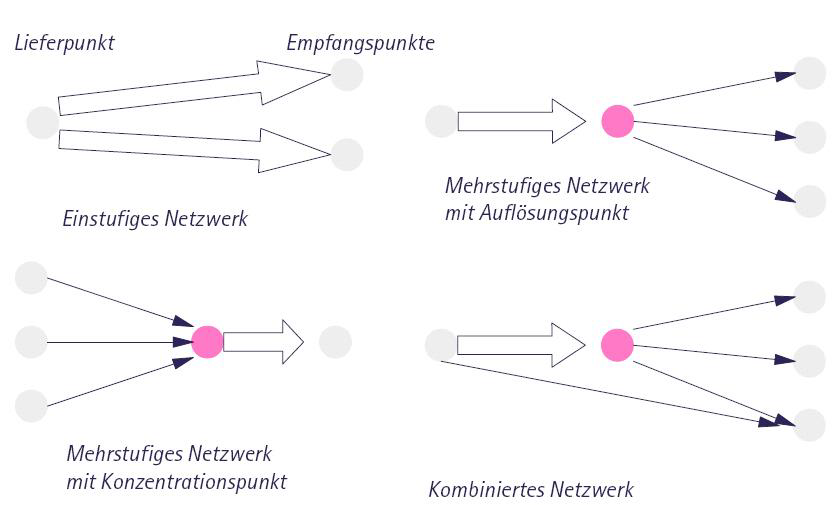
\includegraphics[width=0.7\linewidth]{./Bilder/KV}
	\end{center}

	\chapter{Transportplanung}
	
	Die Transportplanung bildet ein Element der logistischen Unternehmensplanung und wird gemäß betriebswirtschaftlicher Grundsätze sowie orientiert an unternehmenspolitischen Prinzipien (z. B. Leitbildvorstellungen, Unternehmensphilosophien) durchgeführt. Im Folgenden ist der Transportplanungsprozess von der Festlegung der Planungskriterien, bis hin zur Überwachung in einer Grafik aufgeführt.
	\begin{center}
	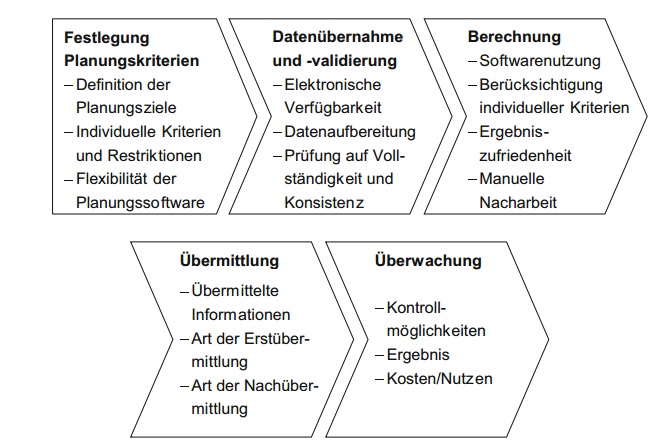
\includegraphics[width=0.7\linewidth]{./Bilder/Transportplanungsprozess}
	\end{center}
	Erklärt beginnt jede Transportplanung mit der Definition von Planungs- bzw. Zielkriterien (z.B. Erreichung eines Servicegrads, Prorisierung von Kunden) sowie die Berücksichtigung vorgegebener Einschränkungen. Die eigentliche Planung dabei beginnt mit der Datenübernahme und -validierung. Diese beinhaltet die Identifikation, Beschaffung und Aggregation sowie Aufbereitung und Prüfung relevanter Daten. Ausgehend von den ermittelten Daten erfolgt die Berechnung von Transportszenarien, -touren und -routen. Im Anschluss daran werden innerhalb des vierten Prozesses die Dokumentation sowie die Übermittlung des Planungsergebnisses an die betreffende Stelle durchgeführt. Obwohl die Überwachung im eigentlichen Sinn keinen Bestandteil der Planungsaufgabe darstellt, ist diese im Rahmen der Transportplanung von elementarer Bedeutung, um die Qualität der Ausführung zu gewährleisten und das Planungsergebnis bewerten zu können.\\
	
	Generell und unabhängig von dem Anwendungsbereich können Transportplanungsprozesse anhand ihrer Laufzeit in strategische, taktische und operative Ebenen gegliedert werden. Der strategische Planungsprozess beinhaltet den Aufbau eines Netzes mit dem Ziel effiziente Transportverbindungen zwischen den Knoten im Planungsgebiet zu schaffen. Auf der taktischen Prozessebene wird die (veränderbare) Gebietsstruktur des Netzwerks festgelegt. Außerdem erfolgt in diesem Zusammenhang die Überplanung von Transportstrukturen und Rahmentouren. Hier dient als Beispiel für die Transporte das Milk-Run Konzept. Es beschreibt die Grundidee, dass Waren in der Menge nur so aufgefüllt werden, wie sie vorher verbraucht worden sind.\\
	
	Auslöser für Überplanungen können Bedarfsänderungen sein, die abweichende Transportmittel und Tarife betreffen. So sind vertragliche Anpassungen häufig in das Aufgabenfeld der taktischen Planung einzuordnen, abhängig von ihrer Vertragsbindung und -dauer können diese jedoch auch Bestandteil der strategischen Transportplanung sein.\\
	
	Im Rahmen der operativen Transportplanungsebene erfolgt die tägliche Durchführung von Dispositionstätigkeiten. Dazu zählt als Kernaufgabe die Koordination und Überwachung der Transporte mit dem Ziel einer kostengünstigen Transportabwicklung bei gleichzeitiger Einhaltung des vertraglich definierten Servicegrads sowie gesetzlicher Bestimmungen (z. B. Lenk- und Ruhezeiten, Zoll- und Gefahrgutvorschriften). In diesem Zusammenhang werden auch die tagesgenaue Touren- und Routenplanung sowie die Transportmittelwahl bzw. Fahrzeugzuweisung durchgeführt. Trotz getrennter Aufgabenbearbeitung innerhalb der drei Ebenen, bedarf es einer Rückkopplung zwischen diesen, um einerseits eine zielgerichtete Umsetzung von Maßnahmen aus der strategischen und taktischen Ebene zu gewährleisten. Andererseits bietet die Rückmeldung aus der Operativen Hinweise für Überplanungen auf der strategischen bzw. taktischen Ebene.\\ 
	
	Trotz eines allgemeinen Transportplanungsansatzes erfordert die Anwendung der Transportplanung auf verschiedene Bereiche die Berücksichtigung charakteristischer Besonderheiten.\\

	\chapter{Planungsmöglichkeiten}
	\section{Manhattan-Metrik}
	Die Manhattan-Metrik ist eine mathematische Möglichkeit um die Effizienz von Transportwegen dahingehend zu erhöhen. Die Formel hierzu sieht folgendermaßen aus:
	\begin{center}
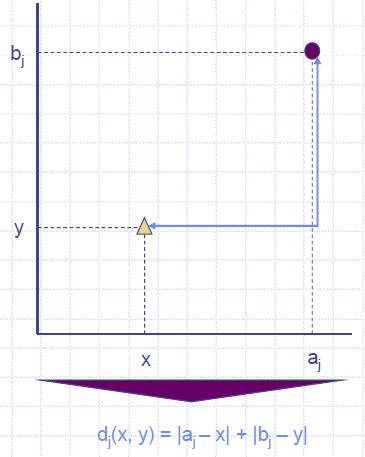
\includegraphics[width=0.5\linewidth]{./Bilder/rechtwinklig}
\end{center}


	Sie beschreibt, dass eine Strecke von A nach B, die Summe aller Teilstrecken, innerhalb eines quadratisch angelegten Straßennetzes darstellt. 
	
	\begin{center}
	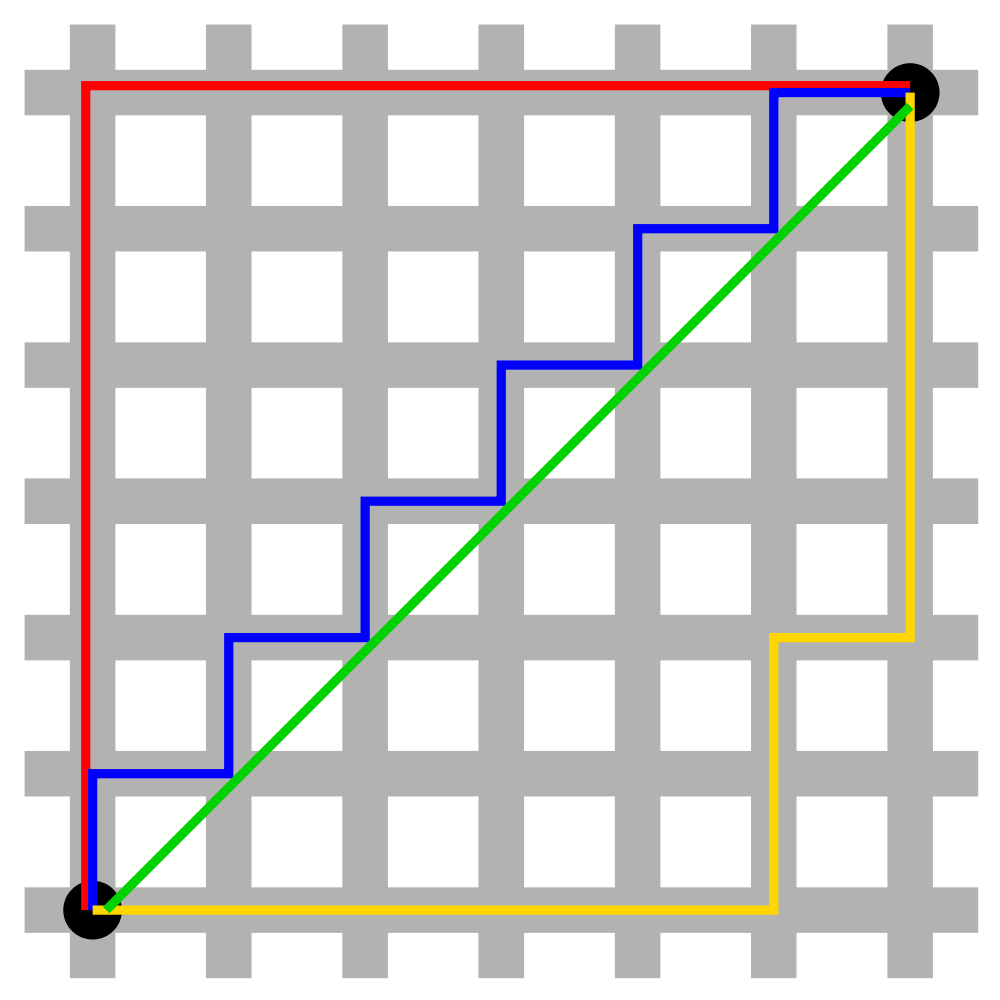
\includegraphics[width=0.5\linewidth]{./Bilder/manhattan}
	\end{center}
	
	Wie der Aufbau der Grafik und der Name bereits vermuten lässt, ist dieses Beispiel von Manhattan, dem Stadtzentrum von New York abgeleitet. Ein LKW-Fahrer der eine Route in solch einem Straßennetz zu bewältigen hat, ist gezwungen diese vertikalen und horizontalen Teilstrecken aneinanderzureihen um ans Ziel zu kommen. Die Linien in rot, blau und gelb sind Beispiele für die Manhattan-Metrik, zwischen den zwei schwarzen Punkten. Die grüne Linie stellt zum Vergleich den Euklidischen Abstand dar. Dieser wird folgendermaßen berechnet:\\
	
	\begin{center}
	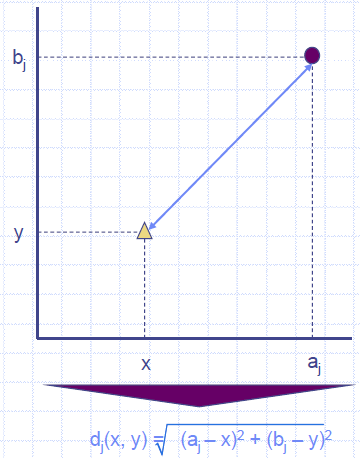
\includegraphics[width=0.5\linewidth]{./Bilder/euklidisch}
	\end{center}

	
	Daher soll die Berechnung der Manhattan-Metrik primär bei der Standortplanung von Logistikverteilzentren und der Planung der einzelnen Transportwege, speziell in Stadtzentren mit ähnlichem Aufbau dienen. Dies geschieht dadurch, dass die einhergehenden Berechnungen mit der Formel der Manhattan-Metrik stark vereinfacht werden können. 
	
	\section{Französische Eisenbahn-Metrik}
	Die Französische Eisenbahn-Metrik ist ein weiteres Beispiel für eine Metrik, die auch in der Logistik Anwendung findet. Sie beschreibt eine bestimmte Anzahl an Punkten X die um einen Punkt P herum verteilt liegen. Die Formel dazu sieht folgendermaßen aus:
	\begin{center}
	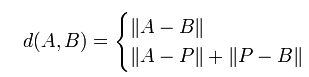
\includegraphics[width=0.7\linewidth]{./Bilder/Formel_Franzoesische_Eisenbahnmetrik}
	\end{center}
			
		Erklärt bedeutet diese Formel, dass eine Direktverbindung zwischen A und B nur möglich ist, wenn P ebenfalls auf der Geraden liegt. Andernfalls muss zuerst die Strecke von A zu P und erst danach kann die Strecke von P zu B absolviert werden.
		
		Das Beispiel leitet sich von dem früher sehr zentralisiert gebauten Eisenbahnnetz von Frankreich ab bei dem alle Bahnverbindungen auf Paris zuliefen.
		Das Problem dabei war nun, dass man bei Reisen zwischen verschiedenen Punkten immer einen langen Umweg über Paris in Kauf nehmen musste, auch wenn die beiden Orte theoretisch direkt nebeneinander liegen.
		\begin{center}
		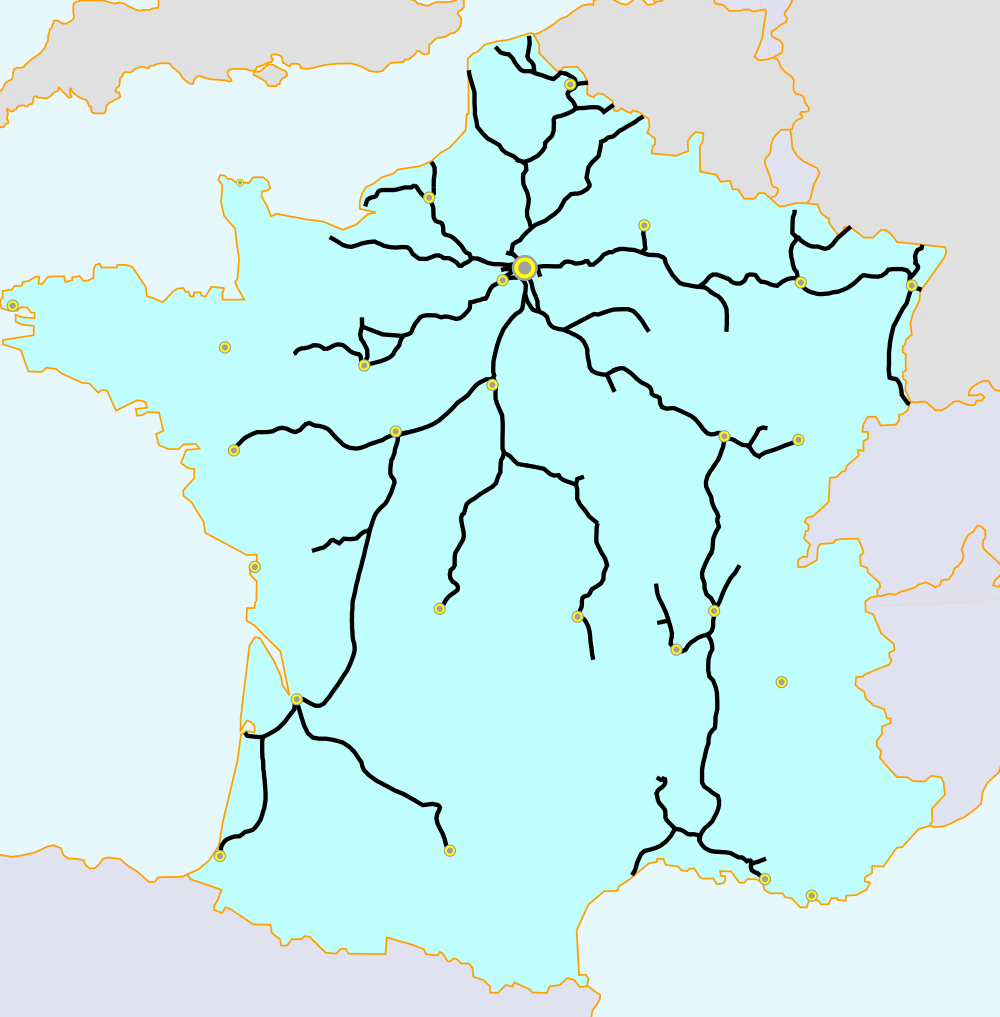
\includegraphics[width=0.6\linewidth]{./Bilder/french_railway}
		\end{center}
	
	\chapter{Produkte}
	\section{SAP APO}
		Ein Beispiel für eine Steuerungssoftware aus dem Hause SAP. SAP Advanced Planning and Optimization (SAP APO) bietet eine vollständig integrierte Palette von Funktionen, die bei der Planung und Ausführung der Logistikprozesse unterstützen.
		\begin{center}
		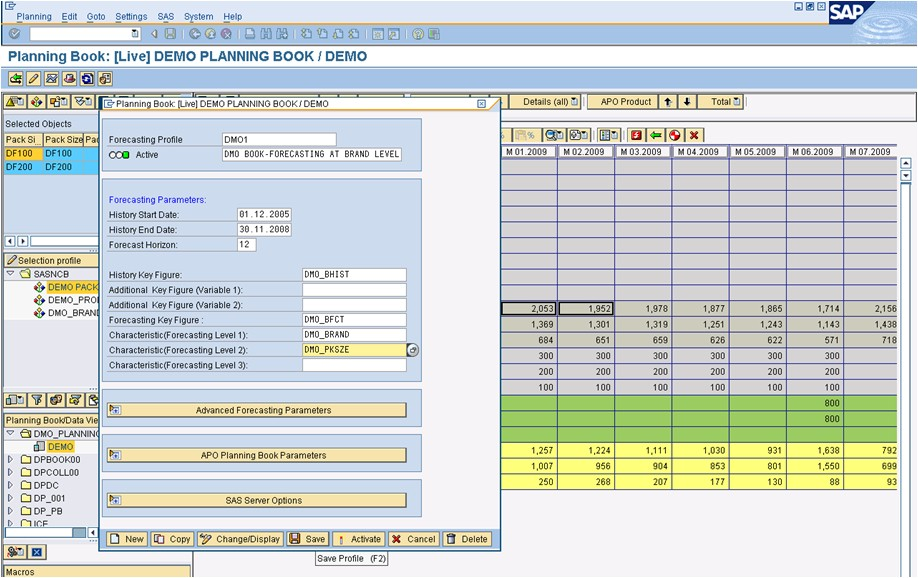
\includegraphics[width=0.7\linewidth]{./Bilder/sas-forecast-SAP-3-full}
		\end{center}


		
	\section{Infor Supply Chain Execution}
		Infor Supply Chain Execution integriert Warehouse-Management, Transportmanagement und andere Aufgabenfelder. Es automatisiert und vereinfacht komplexe Transportmanagementprozesse. 
		\begin{center}
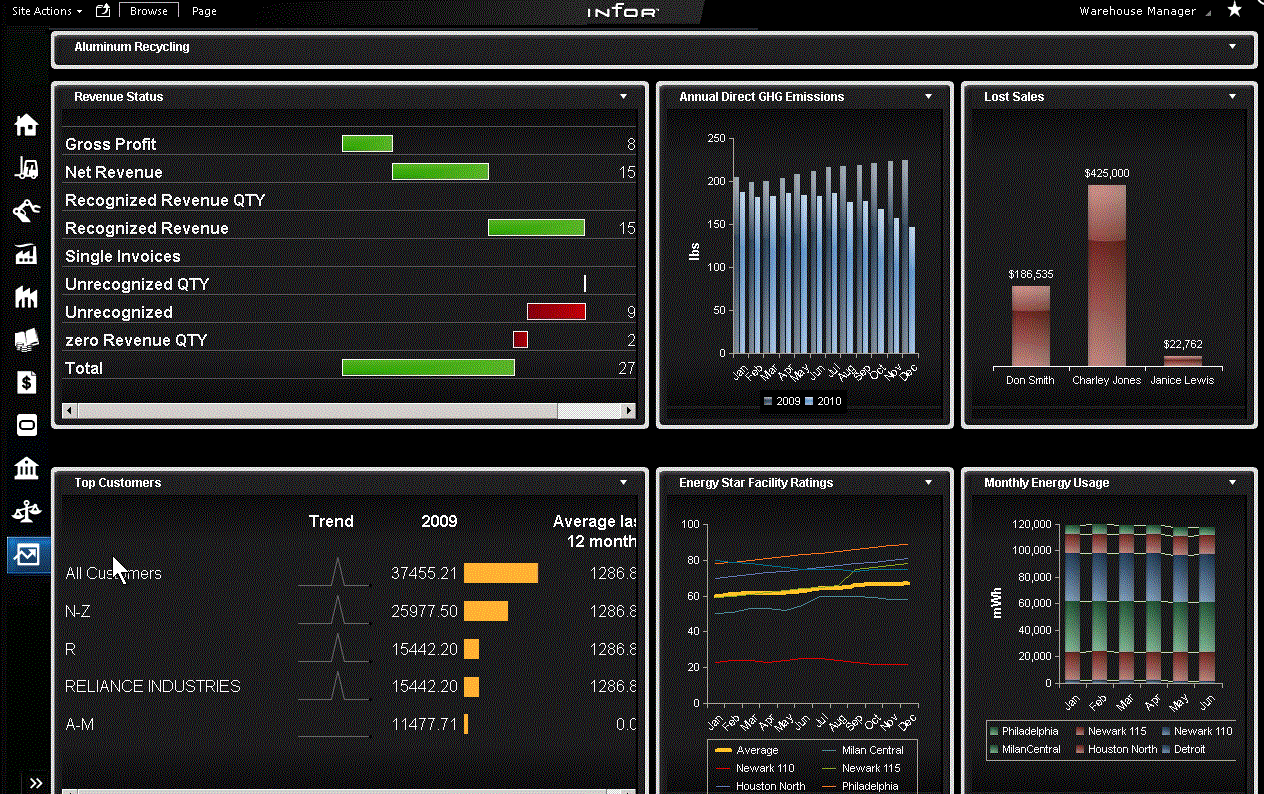
\includegraphics[width=0.7\linewidth]{./Bilder/execution-screenshot1}
\end{center}

		
\chapter{Quellen} 
(1) \nolinkurl{http://de.wikipedia.org/wiki/Transportlogistik}\\
(2) Delfmann W (2008) Kernelemente der Logistikkonzeption. In: Klaus P, Krieger W (eds) Gabler
Lexikon Logistik, 4th edn. Gabler, GWV Fachverlage, Wiesbaden, pp 263-267\\
(3) U. Clausen, C. Geiger (Hrsg.),Verkehrs- und Transportlogistik, Springer-Verlag Berlin\\
(4) \nolinkurl{https://www.firmenkunden.commerzbank.de/files/sector_reports/bb_transport.pdf}\\
(5) Enterprise Resource Planning - ERP Grundlagen, Helmut Vana\\
(6) Produktionsmanagement (Operationsmanagement) - Standortplanung, Helmut Vana
(7) Baumgarten H. (Hrsg.): Das Beste der Logistik; Springer\\
(8) \nolinkurl{https://www.destatis.de/DE/ZahlenFakten/Wirtschaftsbereiche/TransportVerkehr/Gueterverkehr/Tabellen/Gueterbefoerderung.html}\\
(9) \nolinkurl{http://de.wikipedia.org/wiki/Französische_Eisenbahnmetrik}\\
(10) \nolinkurl{http://de.wikipedia.org/wiki/Manhattan-Metrik}
(11) BretzkeWR (2010) Logistische Netzwerke. Springer-Verlag, Berlin, Heidelberg
(11)\nolinkurl{http://www.infor.com/product_summary/scm/sce-logistics-service-providers/}
(12)\nolinkurl{http://help.sap.com/saphelp_scm70/helpdata/de/7e/63fc37004d0a1ee10000009b38f8cf/frameset.htm}


\end{document}